\section{Part 4: Muscle Signal (EMG)}

\begin{taskbox}[Part 4: introduction in the lab manual]
Three EMG segments recorded from three subjects using needle electrodes are provided in the file \texttt{sig\_EMG.mat}. The signals were sampled at 50~kHz and the sampling frequency was then reduced to 4~kHz. One segment belongs to a healthy subject and the other two belong to two patients (Neuropathy and Myopathy). More details about the data can be found at \url{https://archive.physionet.org/physiobank/database/emgdb}.
\end{taskbox}

\subsection{Question 1: Displaying Three Subjects and Examining Waveform Shape at Several Times}
\begin{taskbox}
Plot the time-domain signal of each of the three subjects. Zoom on the horizontal axis in different parts of the signal, examine the features of each signal, and compare them with each other.
\end{taskbox}

Three segments from subjects labeled healthy, myopathy and neuropathy were analyzed. The recordings are of the needle type and, in the version of the data used in this experiment, have a sampling rate of 4000~Hz. According to the official description of the source, the needle electrode was placed in the tibialis anterior muscle, and the original recording was made during mild contraction while lifting the foot against resistance; the original rate of 50~kHz was then reduced to 4~kHz.

The lengths of the recordings are not equal: healthy 12.715~s, myopathy 27.584~s and neuropathy 36.9645~s. Figure~\ref{fig:emgfull} shows all the data with a common scale. The empty space after the end of each recording means that there is no data; it must not be interpreted as muscle silence or zero activity. In the neuropathy recording, transients of larger amplitude are prominent.

\begin{figure}[H]
\centering
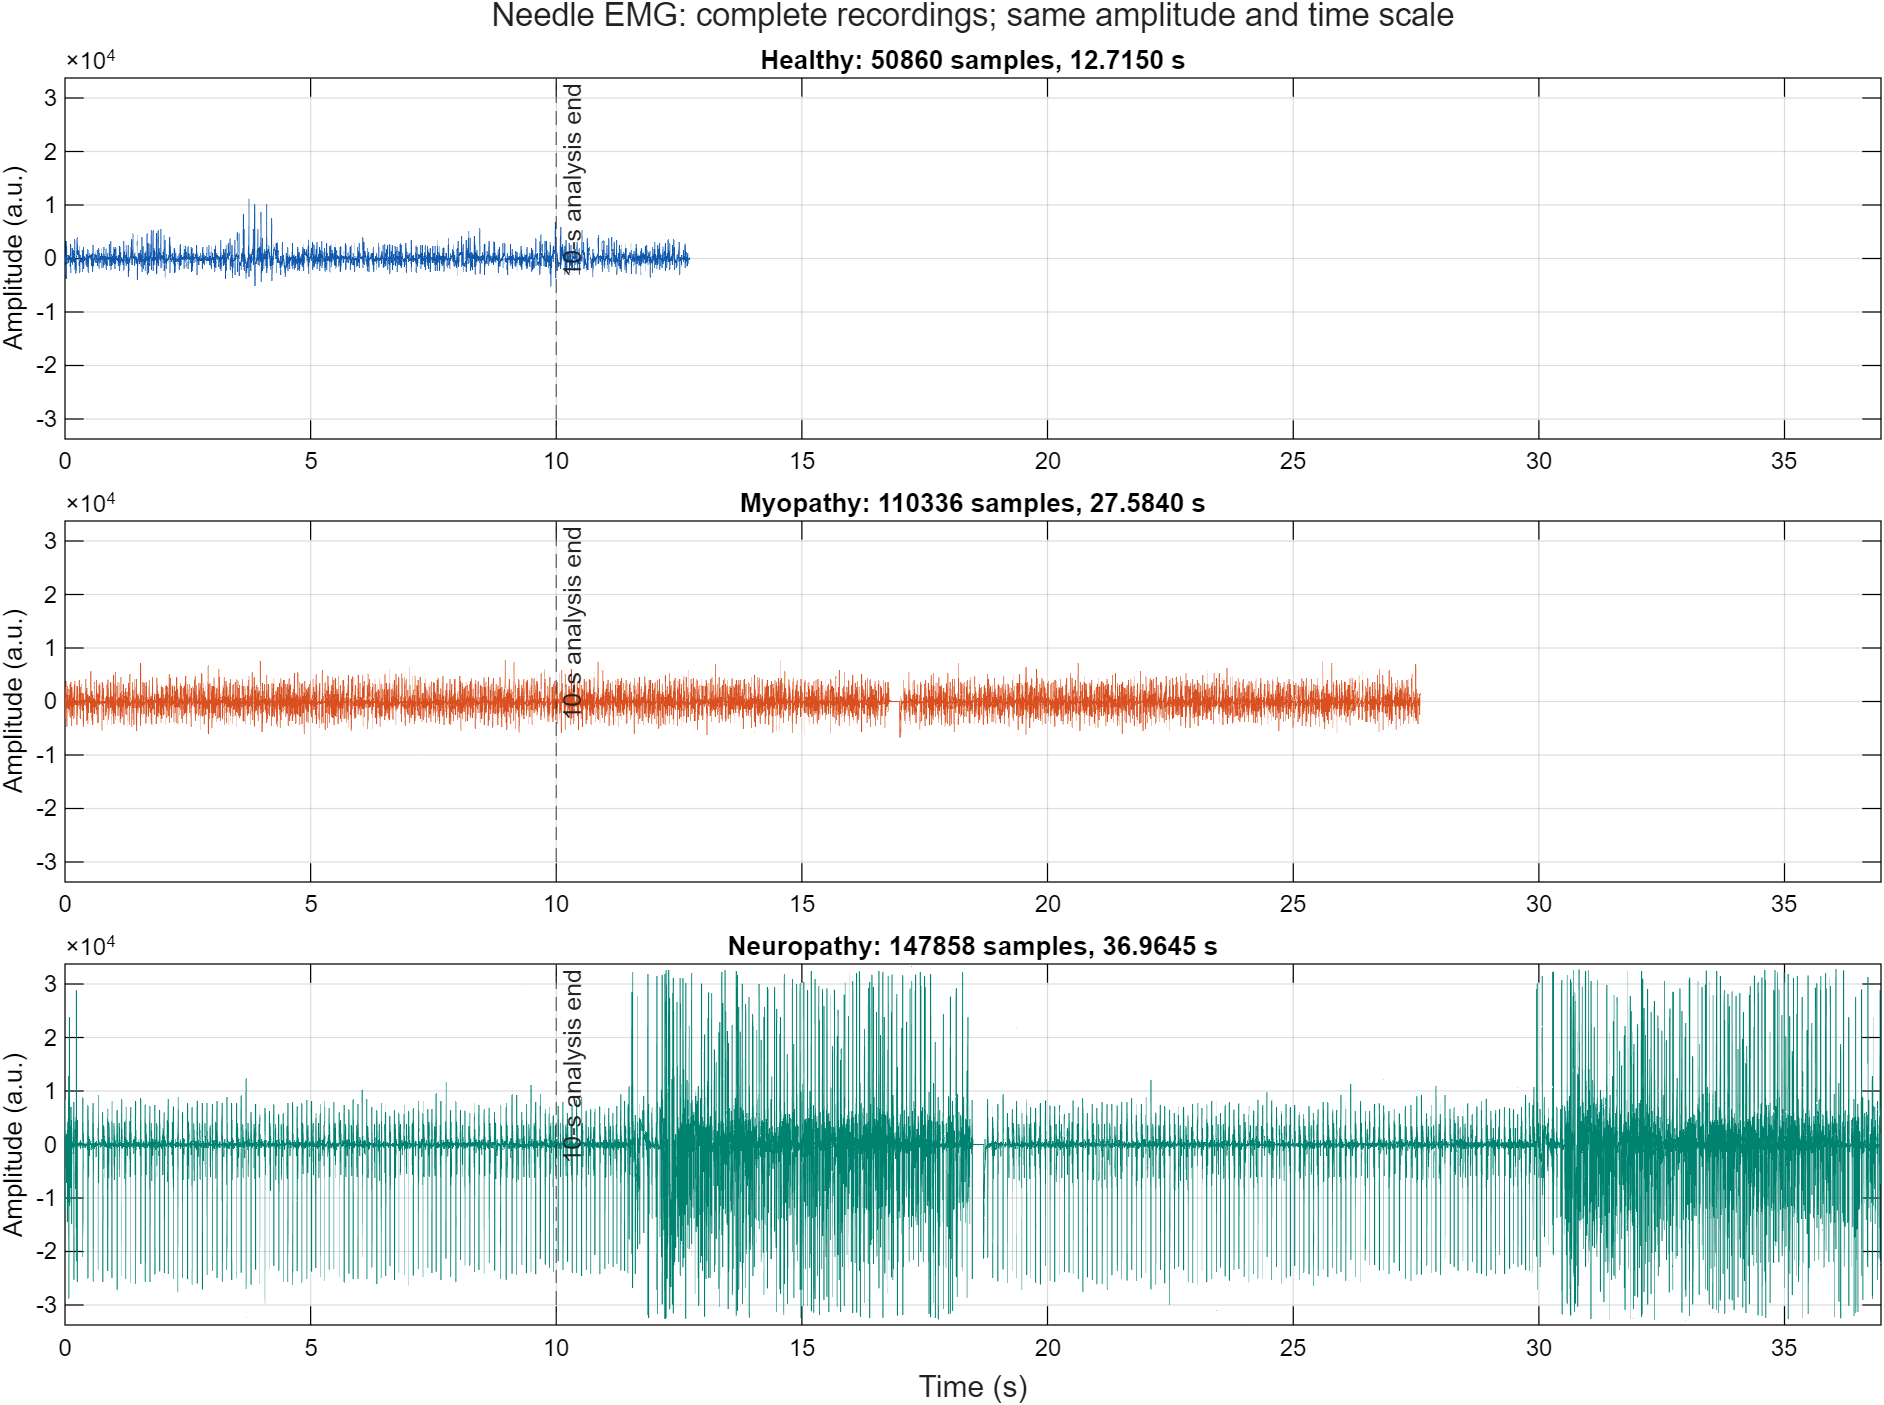
\includegraphics[width=0.95\textwidth]{fig25_emg_full_recordings.png}
\caption{Complete recordings of the three muscle samples with identical time and amplitude axes.}
\label{fig:emgfull}
\end{figure}

For the numerical and spectral comparison, only the first 10 seconds of each recording, i.e.\ 40000 common samples, were selected. Figure~\ref{fig:emg10} shows these intervals on an identical amplitude scale. The stored amplitudes were kept raw; the exercise file has no calibration. The headers of the original database give a factor of 10000~ADC/mV, but the complete equality of the versions, especially the one-sample difference in the original myopathy file, is not proved by the exercise file itself; the unit of the plots is therefore a.u.

\begin{figure}[H]
\centering
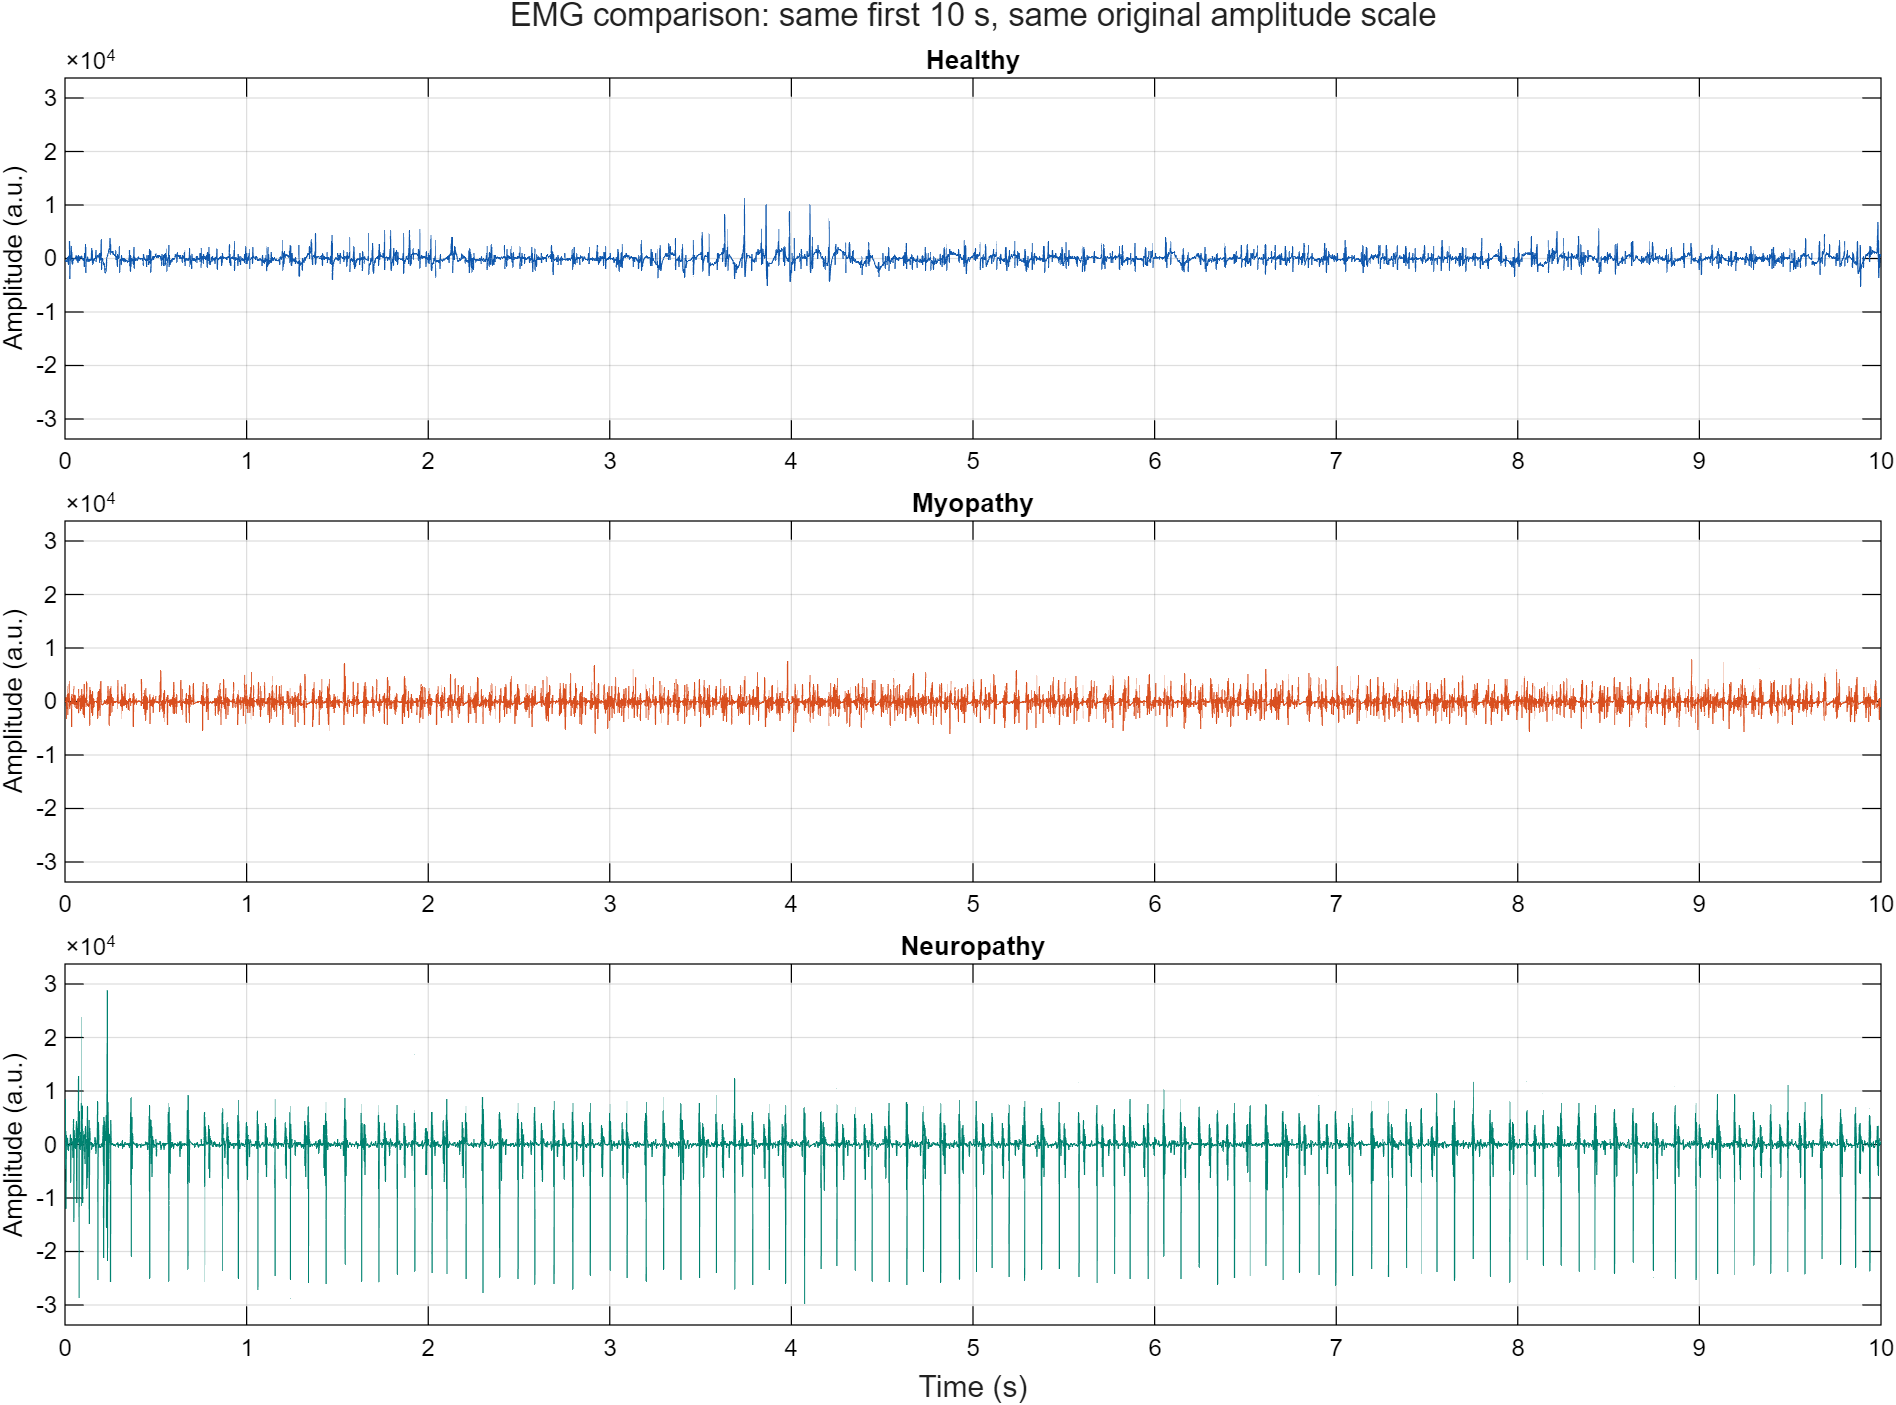
\includegraphics[width=0.95\textwidth]{fig26_emg_first_10s.png}
\caption{Comparison of the first ten seconds of all three recordings without amplitude normalization.}
\label{fig:emg10}
\end{figure}

To examine the local morphology, the intervals 1--1.2, 5--5.2 and 10--10.2~s were zoomed. Figure~\ref{fig:emgzoom} shows that the difference in amplitude and in the density of the transients cannot be determined from the whole recording alone; sharp potentials and local changes of shape are also important. In these samples, the large transients of neuropathy and the denser activity in parts of myopathy can be observed. Since the signal is the sum of several motor units, we do not attribute each peak to a single motor unit without separation.

\begin{figure}[H]
\centering
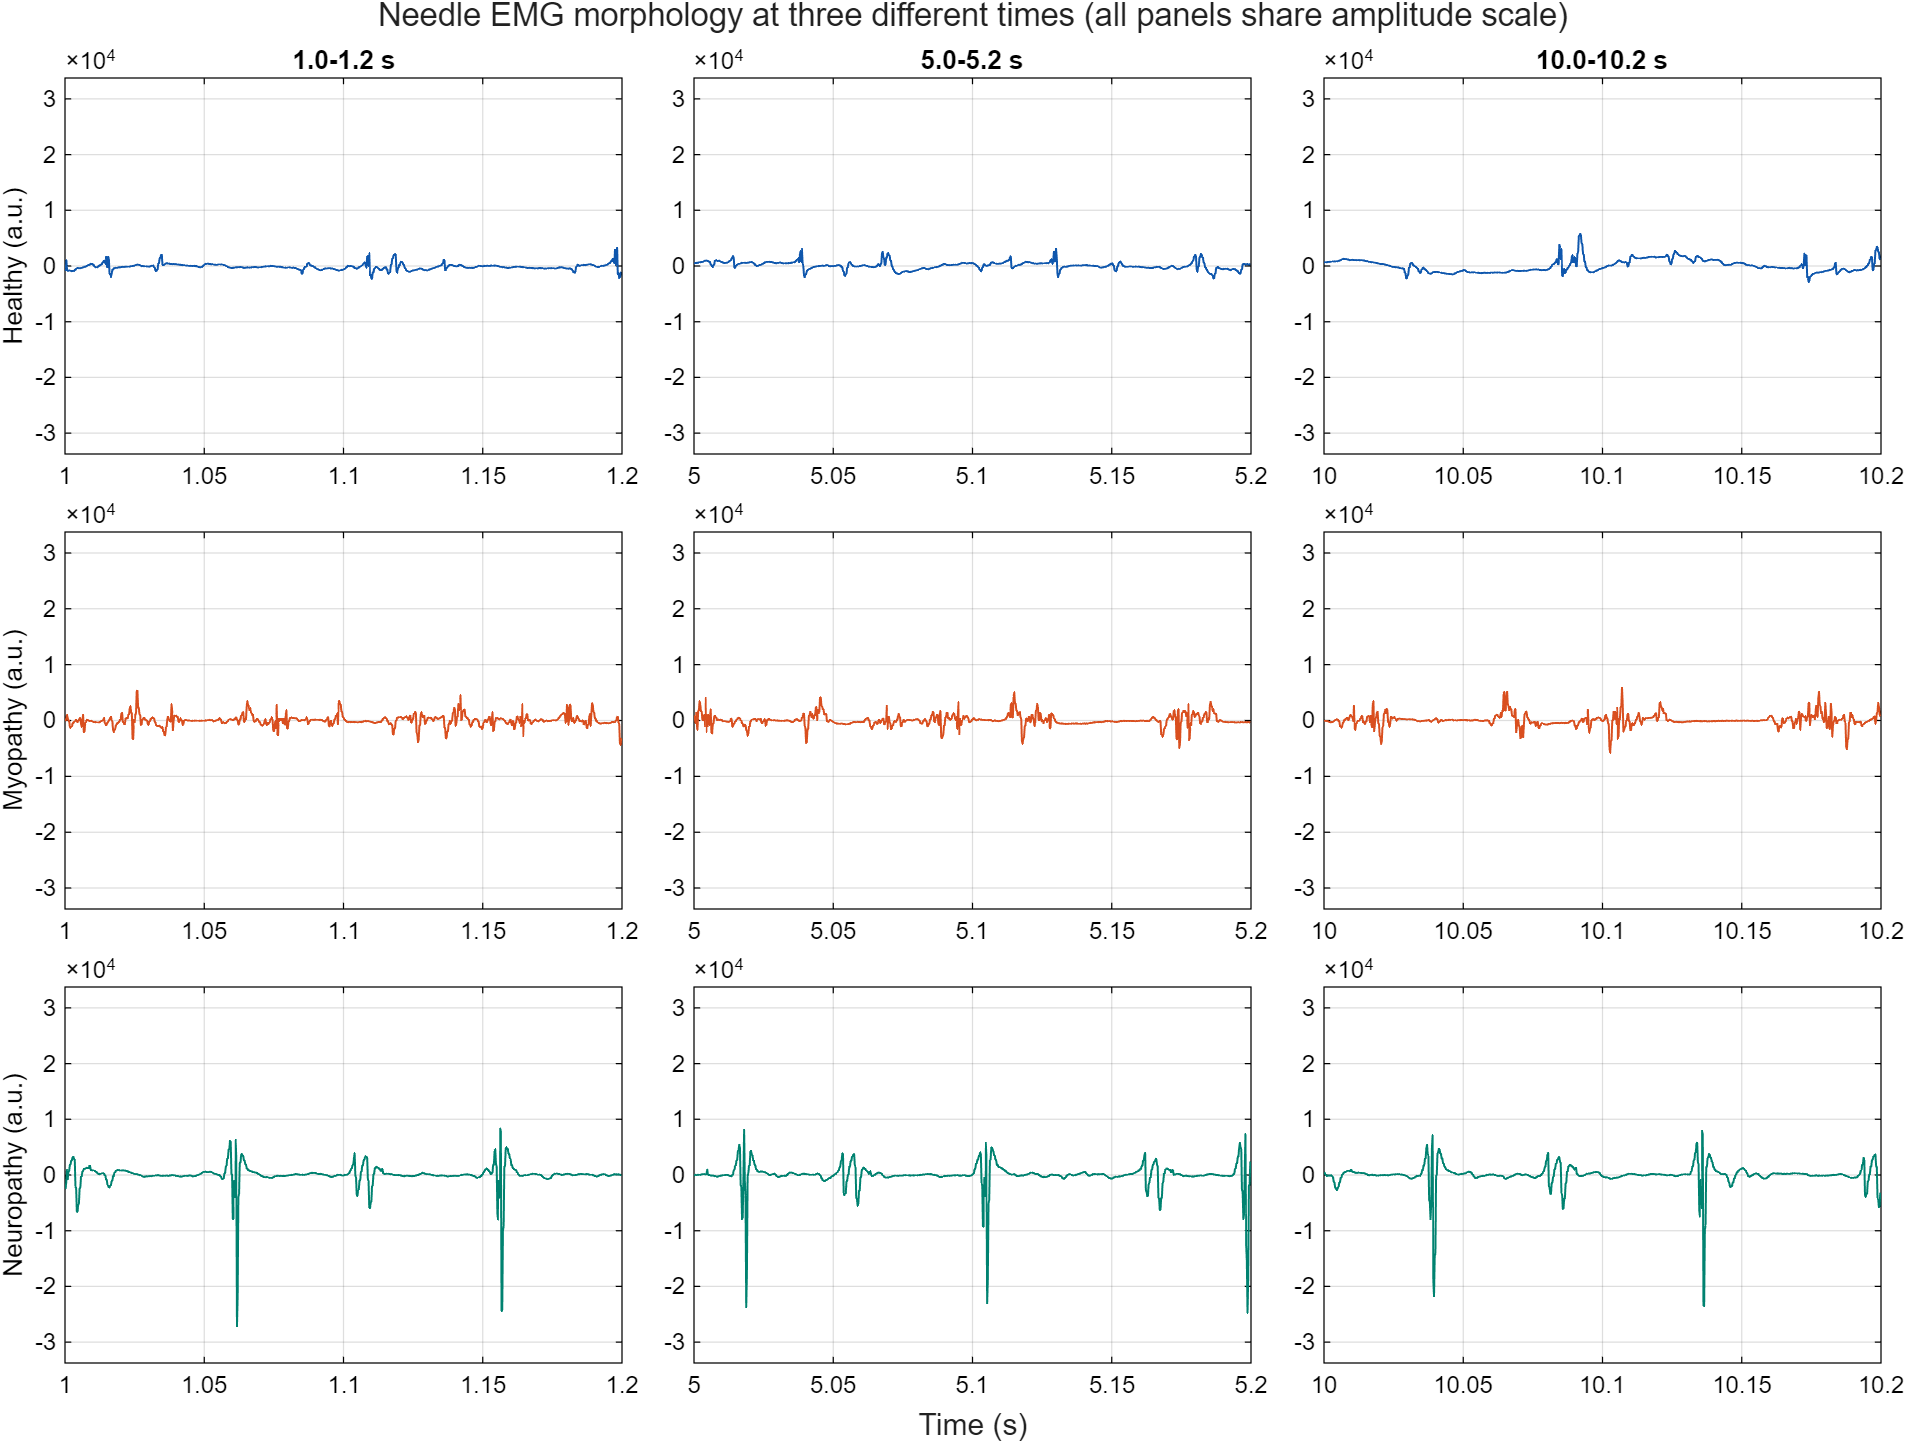
\includegraphics[width=0.95\textwidth]{fig27_emg_local_morphology.png}
\caption{Zoom on three short intervals of each subject, with a common amplitude axis.}
\label{fig:emgzoom}
\end{figure}

\subsection{Question 2: Frequency Spectrum and Spectrogram}
\begin{taskbox}
Plot the frequency spectrum and the time--frequency spectrum of the signal of each subject and compare them with each other.
\end{taskbox}

The Fourier transform and Welch's method were applied to the common ten-second interval after removing the mean. The spacing of the DFT is 0.1~Hz. Welch's estimate was computed with a Hann window of 1024 samples, i.e.\ 256~ms, an overlap of 512 and \texttt{nfft=4096}. Figure~\ref{fig:emgspec} shows both the absolute spectrum and the spectrum with unit area; the first compares the amplitude and power of the recordings, and the second separates the shape of the frequency distribution from the total power.

\begin{center}
\begin{tabular}{@{}lccc@{}}
\toprule
\textbf{Condition} & \textbf{AC RMS} & \textbf{Mean frequency (Hz)} & \textbf{Median frequency (Hz)}\\
\midrule
Healthy    &  820.08 & 166.49 &  63.31\\
Myopathy   &  962.72 & 429.21 & 238.52\\
Neuropathy & 2325.40 & 476.86 & 346.40\\
\bottomrule
\end{tabular}
\end{center}

The mean and the median frequency were computed from the power density:
\begin{equation}
\mathrm{MNF}=\frac{\int_{0}^{f_s/2} f\,P(f)\,df}{\int_{0}^{f_s/2}P(f)\,df},\qquad
\int_{0}^{\mathrm{MDF}}P(f)\,df=\frac12\int_{0}^{f_s/2}P(f)\,df .
\label{eq:mnf}
\end{equation}

\begin{figure}[H]
\centering
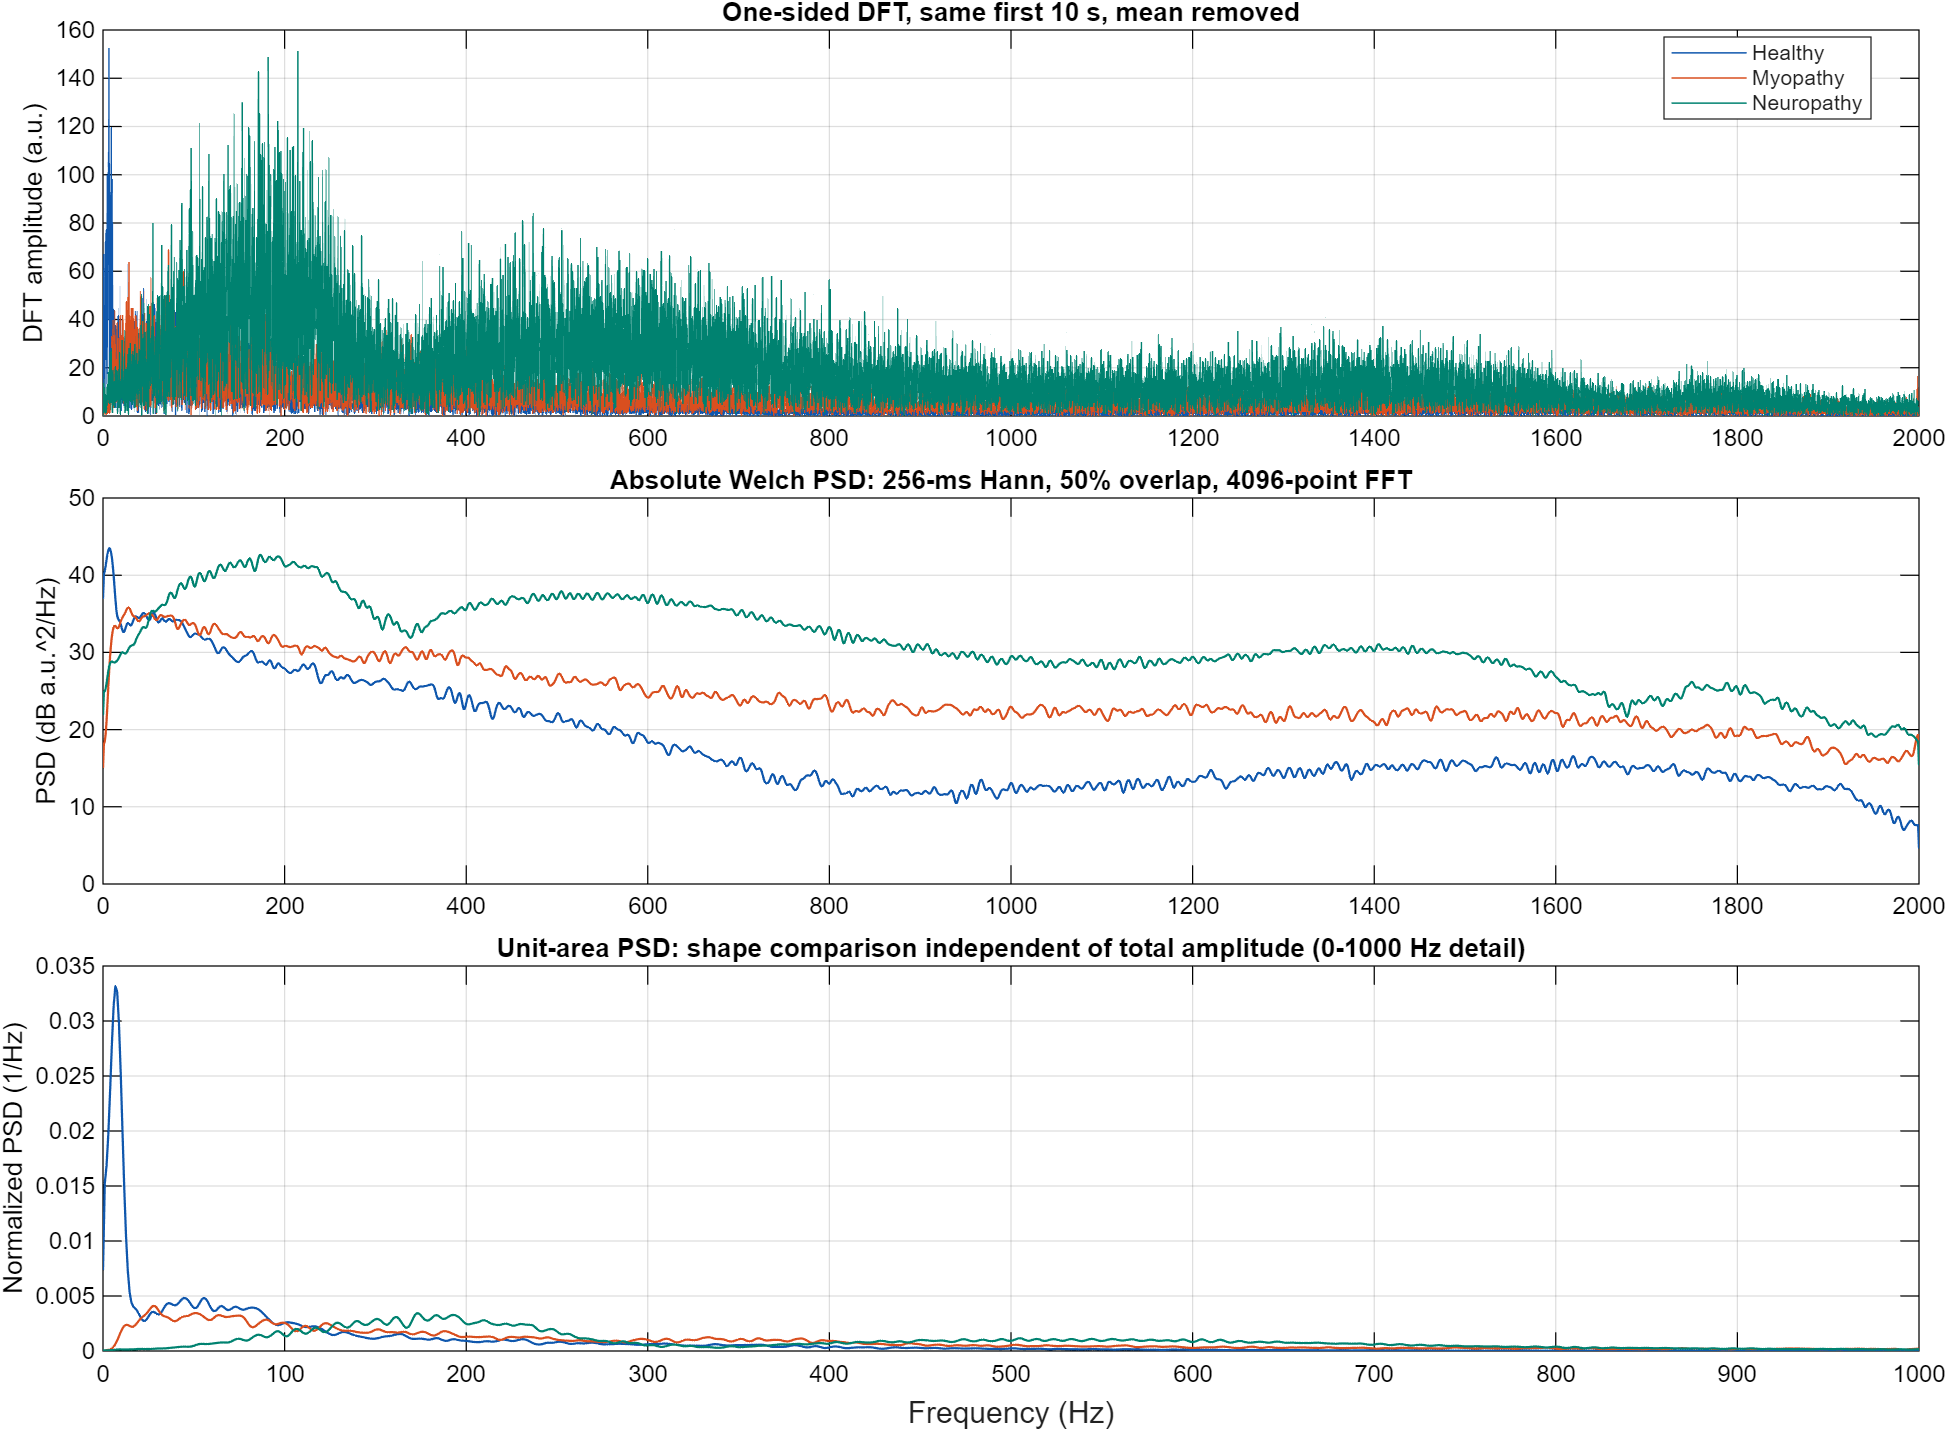
\includegraphics[width=0.95\textwidth]{fig28_emg_spectra.png}
\caption{Absolute amplitude spectrum and power density, and the unit-area power density, in the three muscle recordings.}
\label{fig:emgspec}
\end{figure}

In the present data, the RMS of myopathy is slightly greater than that of the healthy subject, and the RMS of neuropathy is much greater. This experiment is therefore not consistent with the claim that ``the total amplitude of myopathy is always smaller than that of a healthy subject.'' The mean and median frequencies of myopathy and neuropathy are also higher than those of the healthy sample. The Welch peak is about 6.84~Hz for the healthy subject, 28.32~Hz for myopathy and 172.85~Hz for neuropathy; the location of the peak is not the same as the center of mass of the spectrum or the firing rate of a single motor unit. Contraction, the location of the needle, the composition of the units and the quality of the recording also affect these indices.

In the complete neuropathy recording there are five samples with an absolute value of at least 32700, and its minimum is $-32767$. This closeness to the limit of a 16-bit integer raises the possibility of saturation, but by itself it is not proof of amplitude clipping. This issue can affect the amplitude and the fast content of the spectrum. The present analysis neither hid nor removed these samples.

In Figure~\ref{fig:emgstft}, a Hann window of 512 samples, i.e.\ 128~ms, an overlap of 448 samples and \texttt{nfft=2048} was used. The changes in energy intensity and the temporal transients show that the activity is not completely stationary. In neuropathy, more high-power, wide-frequency events are seen, and in the other two recordings the distribution of power over time has a different shape. The region after the end of the healthy or myopathy recording simply has no data. The Nyquist frequency of the present signal is 2000~Hz; the cutoff frequency of the analog filter of the original recording must not be taken as the Nyquist limit of the current version.

\begin{figure}[H]
\centering
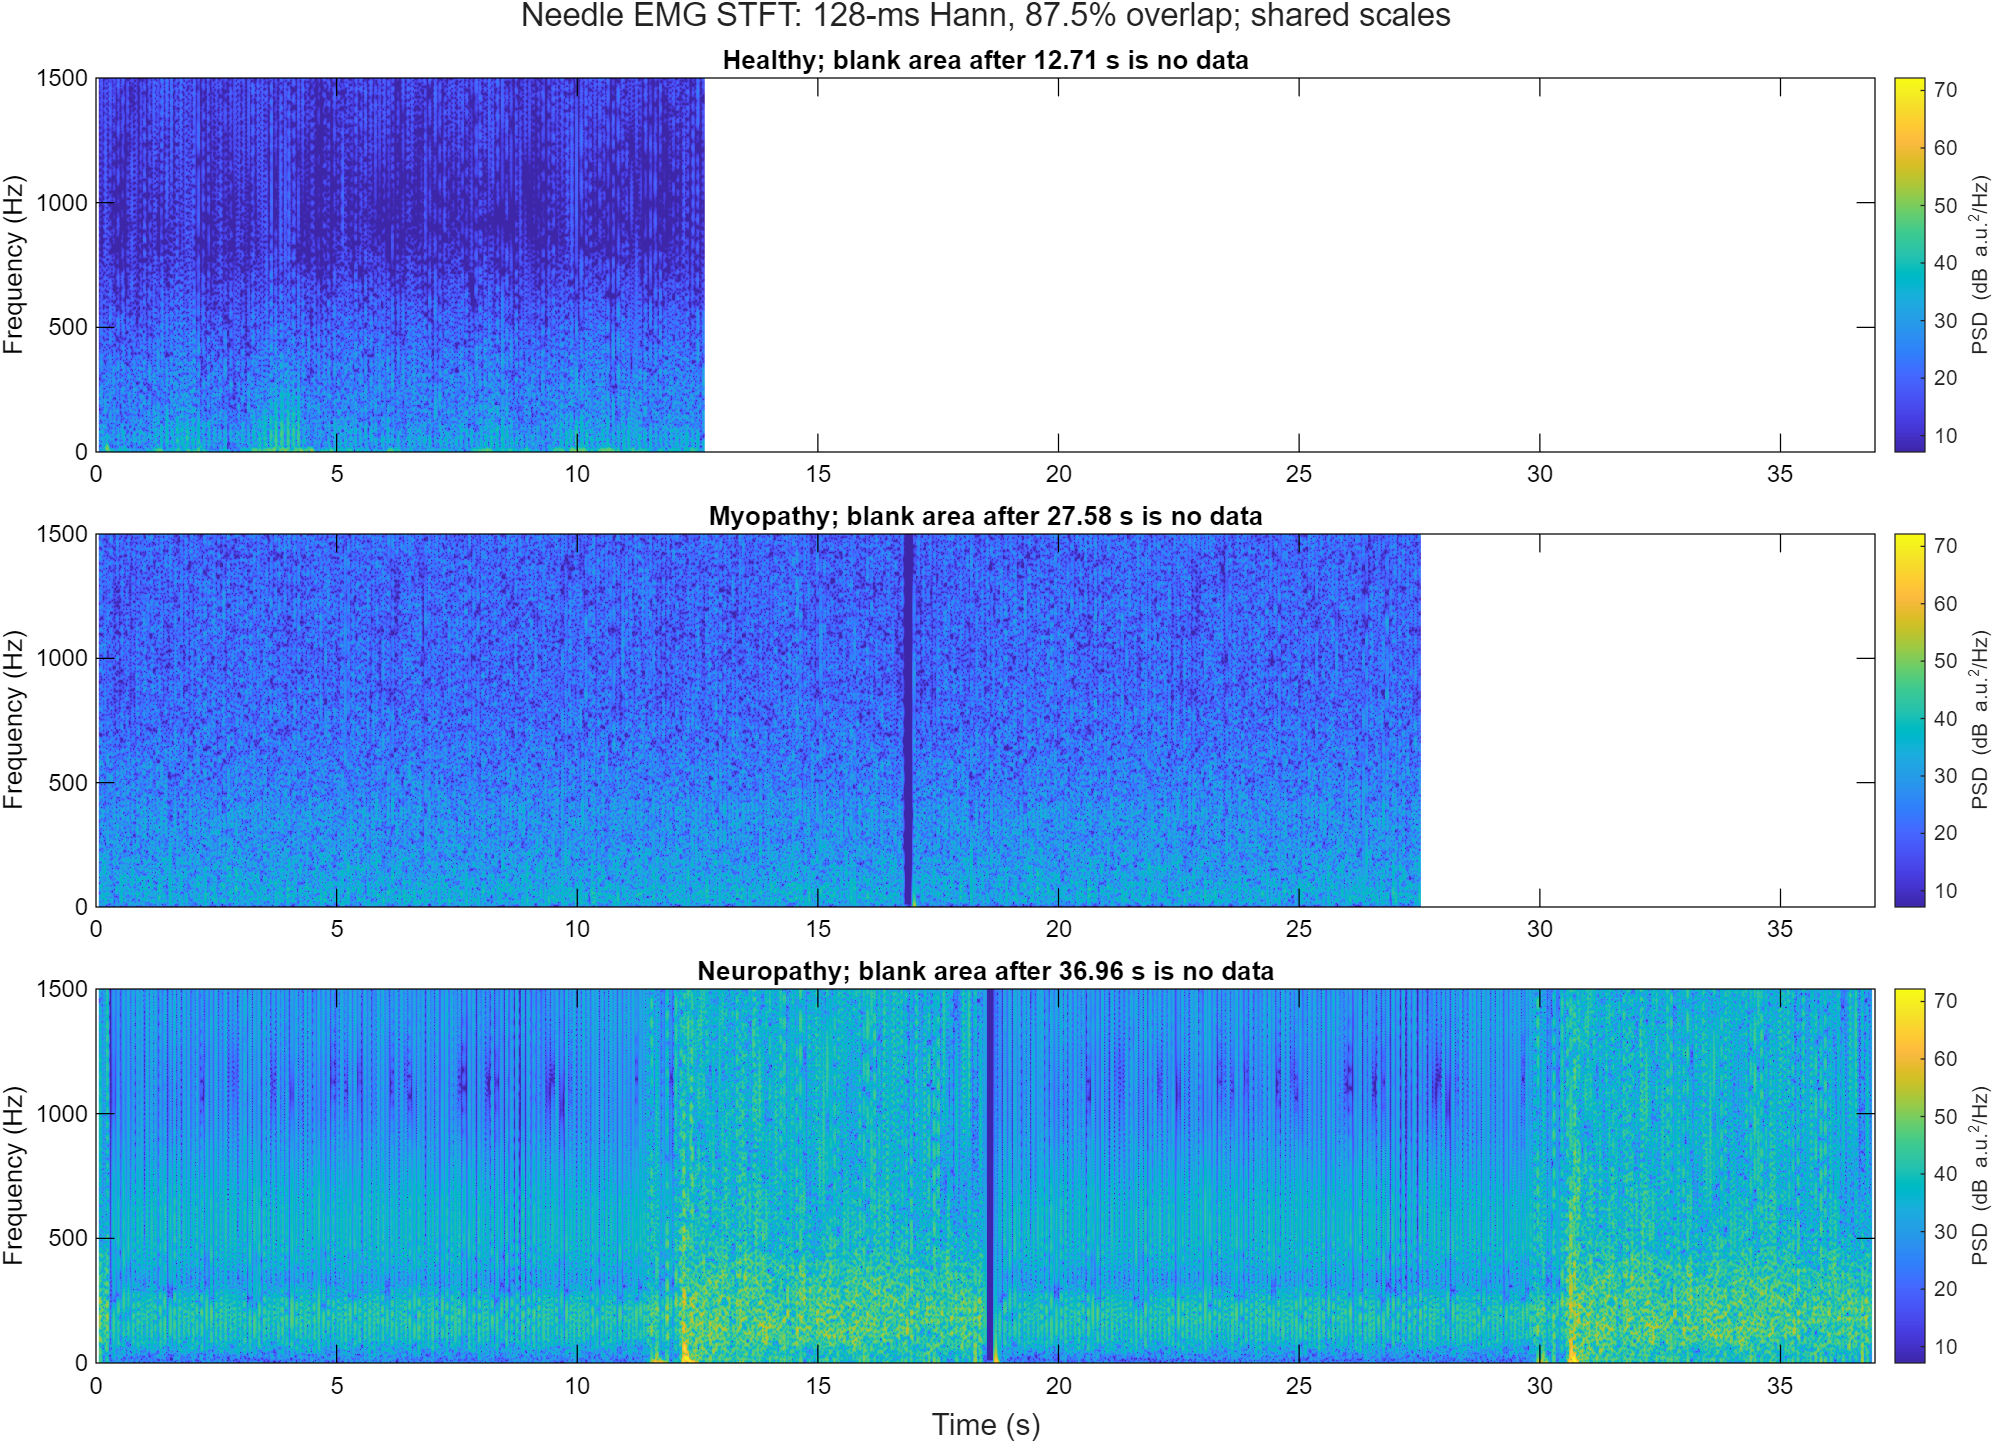
\includegraphics[width=0.95\textwidth]{fig29_emg_stft.png}
\caption{Spectrogram of the complete recordings of the three subjects with common time and frequency axes and common color limits.}
\label{fig:emgstft}
\end{figure}

\subsection{Question 3: Relating the Results to Neuropathy and Myopathy}
\begin{taskbox}
By studying the two diseases, Neuropathy and Myopathy, explain the results obtained in Questions 1 and 2.
\end{taskbox}

A motor unit consists of a motor neuron and the muscle fibers innervated by it, and the recorded signal is the sum of the potentials near the needle. In neuropathy, the main damage is in the nerve or the axon. In chronic neural damage, a reduction in the number of units and collateral reinnervation by the surviving axons can create larger units with longer, higher-amplitude potentials. This process is consistent with the larger transients in the present neuropathy recording, but to prove it, the potentials of the units must be analyzed individually.

In myopathy, the main damage is in the muscle itself. Damage to, or a reduction of, the active fibers of each unit can create shorter, smaller and shape-changed potentials. Nevertheless, the feature of the whole mixed signal is not the same as the characteristic of a single motor unit potential, and analyzing several potentials is important for drawing conclusions. In this experiment, separating the units and measuring the contraction force were not done; therefore the RMS or the median frequency of the three subjects is not a general diagnostic criterion for disease.

The larger transients in the neuropathy sample are consistent with changes in the motor units, but this cannot be proved from the spectrum alone. The myopathy data, in spite of an RMS slightly greater than that of the healthy subject, have a different shape and frequency distribution; this result shows that rules about the amplitude and duration of a single motor unit must not be generalized directly to the total power of the signal. The disease labels come from the data source and are not the product of a classifier built in this experiment.

\subsection{Core Implementation (EMG)}

\begin{lstlisting}[language=Matlab]
N = round(10*fs);                  % Equal duration for all three records
z = emg_healthym(1:N);
z = z(:)-mean(z);
[P,f] = pwelch(z,hann(1024,'periodic'),512,4096,fs);
normalizedPSD = P/trapz(f,P);      % Shape independent of total power
meanFrequency = trapz(f,f.*P)/trapz(f,P);
\end{lstlisting}

The motivation for choosing ten seconds and area normalization is to remove the differences in segment length from the comparison and to separate the difference in amplitude from the shape of the spectrum. This normalization does not remove the differences caused by the electrode location, the contraction intensity or artifacts. The features are stored in \texttt{results/emg\_features.csv}, and the complete code is in \texttt{code/lab1\_eog\_emg.m}.
